\newpage
\section{Implementation}
The major components of the application included, the database, the phone application and the web application version of the application. The application was implemented without a server. The implementation included a cloud database hosted on a third party computer in this case firebase. The phone application was developed for android phones to target the majority of users on campus as per the client's requirements. The Android application was therefore created in Java. The web application was created using JavaScript. Below follows the discussions of these components together with how the they came about and why they were settled on.

\subsection*{Database}
Firebase, a NoSQL cloud database was used as the database option. 
Since a NoSQL database was used, this means that the data in the database was stored as large JSON documents. This helped in reduce the number of deliverable that were to be delivered and hence aided in helping the developers put more focus into other aspects of the problem spectrum. This also reduced the number of resources required to complete the project. The alternative to this would have required a server and a database. The server would have required to be constantly monitored and always on taking data from users and updating it on the database as well as sending new data to the users. With the current approach, we only have a cloud-hosted database that is hosted on Google servers that both applications will be getting data from and sending data to. The database will handle the updating of all users currently connected to it with the new relevant information and as well on the users request give provide the users with the data to populate the menu. The advantages of this approach include the following:
\begin{itemize}
	\item There is no need for a server since firebase database will be able to act both as a server and as a persistent storage tool at the same time. It will assume the role of the server when it needs update the other clients connected to it of new data changes or send the client the data on the database on opening of the application so as to populate the map. This also means there is no stressing about the hosting environment also.
	\item Firebase provide the connected users with realtime updates. This implies that when a value is updated by one user will be sent immediately to the other connected users.
\end{itemize}
\subsubsection*{Database Design}
 During the development cycle, the database had two main designs that where showed to the client. The first design was based on the miscommunication of the client requirements. In this design, the database only stored Location objects together with the signal strengths recorded for that location were stored. This is shown in the figure below
 \begin{figure}
 	\centering
 	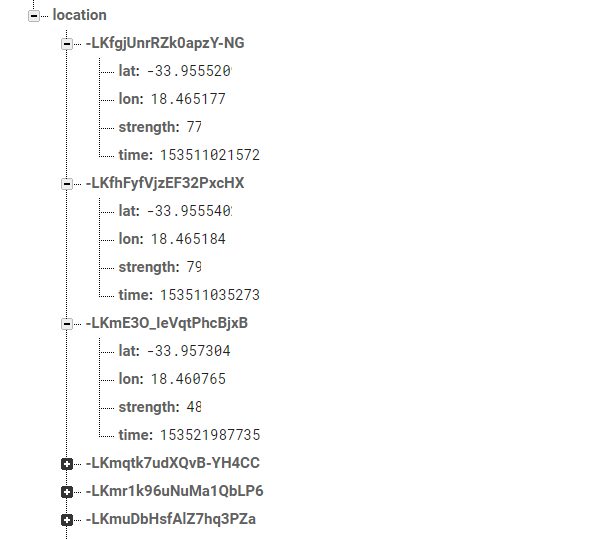
\includegraphics[width=0.7\linewidth]{images/first_db}
 	\caption{Showing the first design of the database developed.}
 	\label{fig:firstdb}
 \end{figure}
As can be seen, there is not much structure in the way the was being stored. Each record had to have an id which made it unique so as to allow better queries. A time stamp was also added to the records on when being written to the database so as to allow future features to use it when they want to filter the strengths based on time. The location was stored as longitude and latitude objects.
\paragraph{}The new database design now also include zone/area objects being stored. This store a list of 4 coordinates that define an area,  the average strength of that area based on location points that are under that area that have recorded data, and lastly the name of the area. This design is shown below in next figure.
\begin{figure}
	\centering
	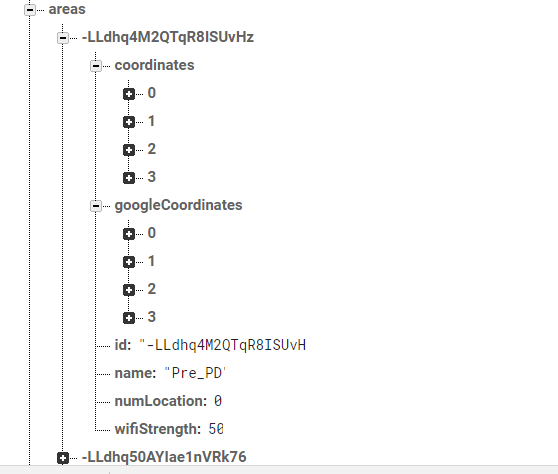
\includegraphics[width=0.7\linewidth]{images/2nd_db}
	\caption[]{Showing the added document for storing area objects.}
\end{figure}
The initial design was still used to maintain the list of all locations that have had data recorded from so as to be able to give the view of the places where the data was recorded for a WLAN zone if needed
Now we get to the details. 

\subsection*{Android application}
The android application was written in Java using the Android Studio tools. The minimum Android version supported in the application was Android 5 API level 21. This version for android was installed in atleast 71\% of the phones of people using android. The reason it was selected to be the minimum supported version was to manage to reach a large population of people at the same time taking advantage of the new features that are in the new APIs which may include better management of resources and security issues for instance. The application built had only one Activity which was the main activity as well. This activity consisted of a map of UCT segmented into different areas based on the buildings and has each color with a specific color that relates into the signal strength in that area. 

\subsection*{Web Application}
Wifi mapper comes with a web client that consists of three views and these are map view, login view and the report view.  

The technologies used to build the app are HTML,CSSS and JavaScript. A few frameworks were also include to improve team productivity.

The map view displays a google map that contains the WLAN ZONEs over UCT upper campus. The app gets the map from the google map api obtained by including a script on the html file of the view.

The map view is set up such that the map fills the screen of the device fully. After rendering the map, the app asynchronously gets data from the firebase database using the 'on' firebase listener. The app sets the location center and defualt zoom. In order to get the data from the database firebase was added as a dependence on the app. 

After obtaining the data from the database, the app displays colored polygons on top of respective WLAN ZONEs. The colors of the polygons are calculated using the data returned by the database. Five colors are used to represent ranges between 0 and 100. 

The map view also contains a button used to generate report for special users. On clicking this button, the login view is displayed on the screen.

The login view consists of a login form with two input fields and a login button. The two input fields are for username and password. The password input field is such that the password is hidden while the user is typing it. 

The login button has an onLogin listener attached to it. When the button is clicked/tapped an onLogin event is fired that sends a request to the server to check if the user is authenticated to view the report. If the user is authenticated then the app displays the wifi mapper report.

The report is used to display special statistics to the user. The app calculates the number of locations and signal strength then displays them at the top of the view. Number of WLAN ZONEs is also calculated and displayed together with the number of locations.

Following the calculated numbers, the report displays bar ,pie and bubble charts for the data on firebase. The first bar chart shows the average wifi strength against the WLAN ZONEs on the map. The bar chart is followed by a pie chart that shows a different representation of the average wifi strength against the WLAN.

The app uses a library called chart.js to convert the data from javascript objects to charts. Calculations for the color are done by a single function for all the charts. The calculation is such the only bright colors are used for all chart components.

The report view was developed using modern frameworks like bootstrap that makes the report responsive accross all devices.

